\documentclass[12pt, twoside]{article}
\usepackage[letterpaper, margin=1in, headsep=0.5in]{geometry}
\usepackage[english]{babel}
\usepackage[utf8]{inputenc}
\usepackage{amsmath}
\usepackage{amsfonts}
\usepackage{amssymb}
\usepackage{tikz}
\usepackage{yhmath}
%\usetikzlibrary{quotes, angles}

\usepackage{graphicx}
\usepackage{enumitem}
\usepackage{multicol}

\usepackage{fancyhdr}
\pagestyle{fancy}
\fancyhf{}
\renewcommand{\headrulewidth}{0pt} % disable the underline of the header

\fancyhead[RE]{\thepage}
\fancyhead[RO]{\thepage \\ Name: \hspace{3cm}}
\fancyhead[L]{BECA / Dr. Huson / 10th Grade Geometry\\* 8 May 2019}

\begin{document}
\subsubsection*{10.10 Pretest: Volume, density, trig review}
 \begin{enumerate}

   \item The area of $\triangle ABC$ is $120.7$ square inches. The altitude $h$ of the triangle is 8.5 inches. Find the length of the base $AB$.\\[0.5cm]
   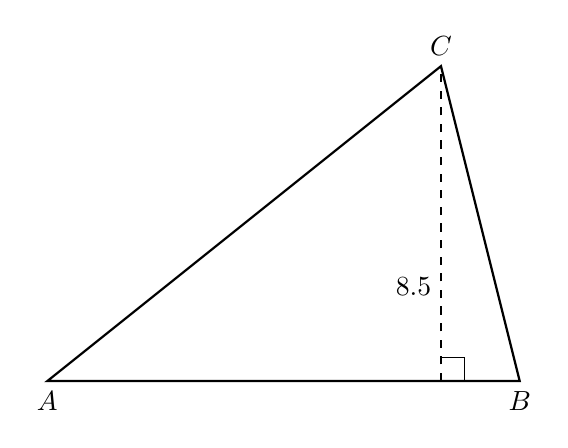
\begin{tikzpicture}[scale=1.0]
     \draw [thick]
       (0,0)node[below]{$A$}--
       (6,0)node[below]{$B$}--
       (5,4)node[above]{$C$} --cycle;
    \draw [dashed] (5,0)--(5,4);
    \draw (5,0)++(0.3,0)--++(0,0.3)--+(-0.3,0);
    \node at (5,1.2)[left]{$8.5$};
    %\node at (3,0)[below]{$20.7$};
  \end{tikzpicture} \vspace{0.5cm}

  \item In a right triangle, the acute angles have the relationship $\sin (2x)=\cos(70)$.\\[0.25cm]
    What is the value of x? \vspace{2.5cm}

  \item If $\sin (8x-8)^\circ = \cos(7x+8)^\circ$, what is the value of $x$? \vspace{3cm}

  \item Write an equation of the line that is perpendicular to the line whose equation is $3y=2x+6$ and passes through the point $(-1,7)$. \vspace{2cm}

  \item Find the distance between $(1,9)$ and $(6, -3)$.

\newpage
  \item From a point on the ground one-half mile from the base of a historic monument, the angle of elevation to its top is $11.87^\circ$. To the nearest foot, what is the height of the monument?\\[1cm]
   \begin{tikzpicture}[scale=1.1]
     \draw [dashed] (10,0)--(0,0)--(10,2);
     \draw [thick, ->] (10,0)--(10,2);
     \draw (10,0)++(-0.3,0)--++(0,0.3)--+(0.3,0);
     \fill [gray] (0,0)--(0.75,0) arc [start angle=0, end angle=11.3, radius=0.75]--cycle;
     \node at (1,0)[below]{$11.87^\circ$};
     \node at (10,1)[right]{Monument};
     \node at (6,0)[below]{One-half mile};
   \end{tikzpicture} \vspace{3cm}

  \item A homeowner is building three steps leading to a deck, as modeled by the diagram below. All three step rises, $\overline{HA}$,  $\overline{FG}$, and  $\overline{DE}$, are congruent, and all three step runs, $\overline{HG}$,  $\overline{FE}$, and  $\overline{DC}$, are congruent. Each step rise is perpendicular to the step run it joins. The measure of $\angle CAB = 36^\circ$ and $\angle CBA = 90^\circ$.\\[0.5cm]
    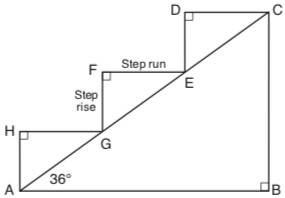
\includegraphics[width=0.4\textwidth]{steps_Aug2018-33.png}\\
  If each step run is parallel to $\overline{AB}$ and has a length of 10 inches, determine and state the length of each step rise, to the \emph{nearest tenth of an inch}.\\[3cm]
  Determine and state the length of $\overline{AC}$, to the \emph{nearest inch}.

\newpage
  \item The secants $\overline{ABC}$ and $\overline{ADE}$ intersect the circle $O$, as shown in the diagram. \\Given $m \wideparen{BD}=30^\circ$ and $m \wideparen{CE}=150^\circ$. Find the $m\angle A$.
       \begin{center}
       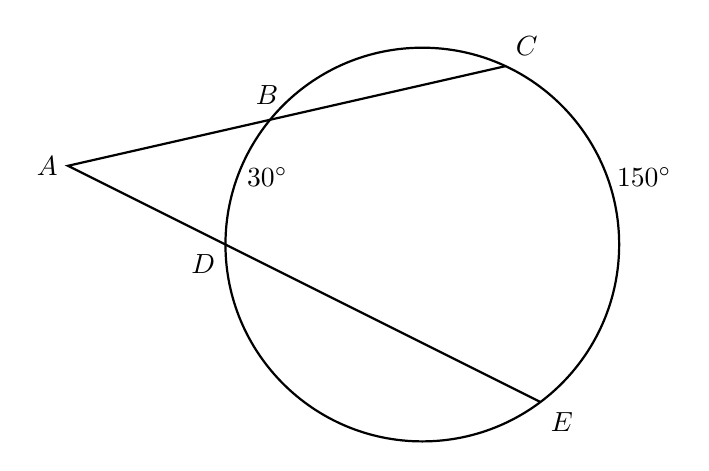
\begin{tikzpicture}[scale=.5]
         \draw [thick] (0,0) circle[radius=5];
         \draw [thick]
         (3,-4) node[below right] {$E$}--
         (-5,0) node[below left] {$D$}--
         (-9,2) node[left] {$A$}--
         (65:5) node[above right] {$C$};
         \draw (132:5.1) node[left] {$B$};
         \draw (20:5) node[right] {$150^\circ$};
         \draw (160:5) node[right] {$30^\circ$};
       \end{tikzpicture}
     \end{center} \vspace{2cm}

  \item The secants $\overline{PQR}$ and $\overline{PST}$ intersect the circle $O$, as shown in the diagram. \\Given $m \angle P=40^\circ$ and $m \wideparen{RT}=140^\circ$. Find the $m\wideparen{QS}$.
       \begin{center}
       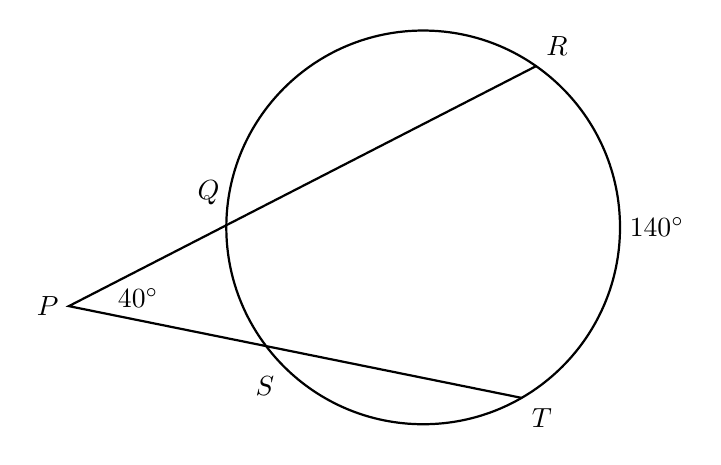
\begin{tikzpicture}[scale=.5]
         \draw [thick] (0,0) circle[radius=5];
         \draw [thick]
         (-60:5) node[below right]{$T$}--
         (-9,-2) node[left]{$P$}--
         (55:5) node[above right]{$R$};
         \draw (225:5) node[below left]{$S$};
         \draw (170:5) node[left] {$Q$};
         \draw (0:5) node[right] {$140^\circ$};
         \draw (-8,-1.8) node[right] {$40^\circ$};
       \end{tikzpicture}
     \end{center} \vspace{1cm}

\newpage
   \item Given circle $Z$ with inscribed $\triangle XYZ$. $m\angle Z=100$. Find $m\angle Y$.\\[1cm]
       %\hspace{1cm} Given the line  $l$ and point $P$.
       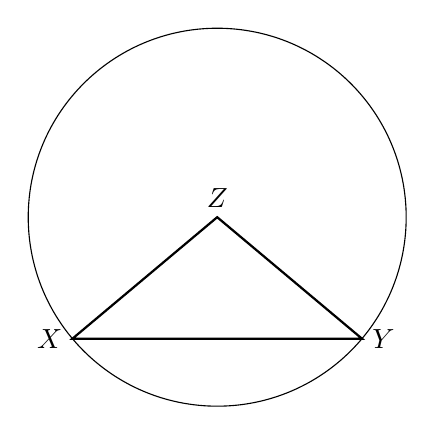
\begin{tikzpicture}[scale=0.8]
         %\draw [-, thick] (-6,0) node[left]{$A$}--(0,0);
         \draw  (0,0) circle [radius=3] node[above]{$Z$};
         \draw [-, thick] (220:3) node[left]{$X$}--(0,0)
           --(320:3) node[right]{$Y$}--cycle;
         %\node at (8.5,-0.4){$l$};
         %\draw [fill] (6,0) circle [radius=0.05] node[below]{$Q$};
       \end{tikzpicture} \vspace{3cm}

     \item Given circle $O$ with inscribed $\triangle SLO$. $m\angle S=x+7$. Find $m\angle O=2x-2$. Find $x$.\\
     For full credit, check your answer.\\[1cm]
         %\hspace{1cm} Given the line  $l$ and point $P$.
         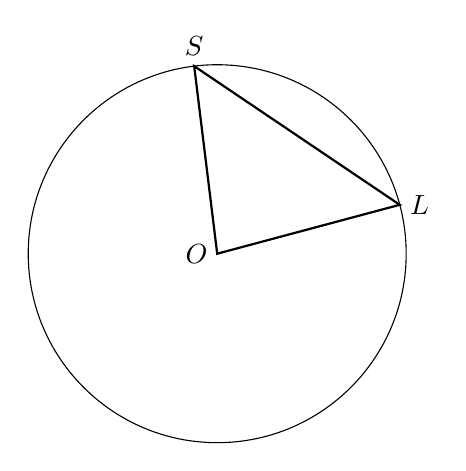
\begin{tikzpicture}[scale=0.8]
           %\draw [-, thick] (-6,0) node[left]{$A$}--(0,0);
           \draw  (0,0) circle [radius=3] node[left]{$O$};
           \draw [-, thick] (15:3) node[right]{$L$}--(0,0)
             --(97:3) node[above]{$S$}--cycle;
           %\node at (8.5,-0.4){$l$};
           %\draw [fill] (6,0) circle [radius=0.05] node[below]{$Q$};
         \end{tikzpicture}


\end{enumerate}
\end{document}


   \item On the set of axes below, $\triangle ABC$, altitude $\overline{GC}$, and  median $\overline{MC}$ are drawn.
    \begin{center}
      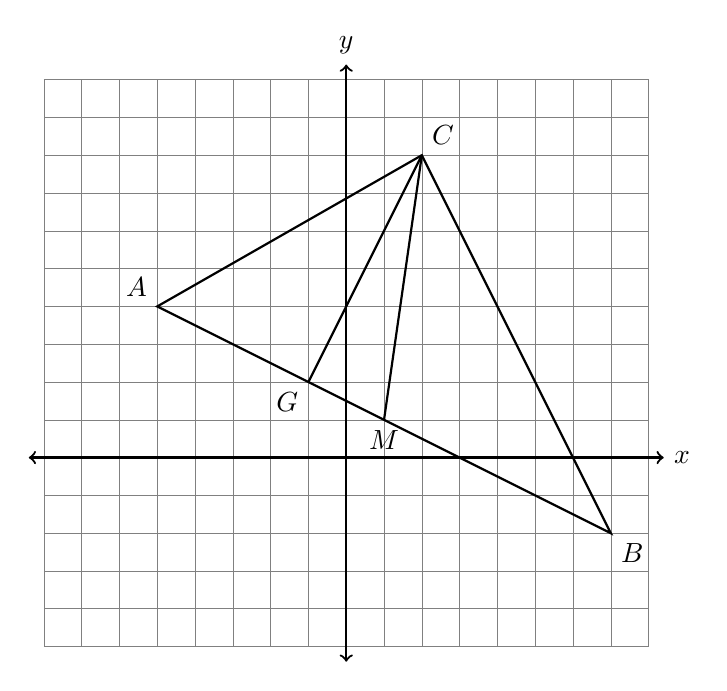
\begin{tikzpicture}[scale=.48]
        \draw [help lines] (-8,-5) grid (8,10);
        \draw [thick, <->] (-8.4,0) -- (8.4,0) node [right] {$x$};
        \draw [thick, <->] (0,-5.4)--(0,10.4) node [above] {$y$};
        \draw [thick]
          (-5,4) node[above left] {$A$}--
          (7,-2) node[below right] {$B$}--
          (2,8) node[above right] {$C$}--
          cycle;
        \draw [thick] (1,1) node[below] {$M$}--(2,8);
        \draw [thick] (-1,2) node[below left] {$G$}--(2,8);
      \end{tikzpicture}
    \end{center}
      Determine which equations represent the area of the triangle, circling True or False.
      \begin{multicols}{2}
       \begin{enumerate}
       \item \quad T \quad F \quad $\displaystyle Area_\triangle = \frac{(AC)(AB)}{2}$ \vspace{0.25cm}
       \item \quad T \quad F \quad $\displaystyle Area_\triangle = \frac{(CG)(BC)}{2}$
       \item \quad T \quad F \quad $\displaystyle Area_\triangle = \frac{(CM)(AB)}{2}$ \vspace{0.25cm}
       \item \quad T \quad F \quad $\displaystyle Area_\triangle = \frac{(CG)(AB)}{2}$
      \end{enumerate}
      \end{multicols}
      \vspace{0.25cm}


        \item The map of a campground is shown below. Campsite C, first aid station F, and supply station S lie along a straight path. The path from the supply station to the tower, T, is perpendicular to the path from the supply station to the campsite. The length of path FS is 400 feet. The angle formed by path TF and path FS is $72^\circ$. The angle formed by path   and path CS is $55^\circ$.\\[0.5cm]
        \includegraphics[width=0.5\textwidth]{camp_Jun2018-31.png}
          \begin{enumerate}
            \item Determine and state the volume of concrete needed, \emph{in cubic feet}. \vspace{1cm}
            \item Sarah can mix her own concrete for \$3.25 per cubic foot. How much money will it cost her to replace the two concrete sections?
        \end{enumerate} \vspace{2.5cm}
